\section{Actividad 11}

\subsection*{Un transmisor de FM tiene el diagrama de bloques que se observa en la Fig.~1. La respuesta de audiofrecuencia es plana sobre la banda de audio de 
$40~\text{Hz}$ a $15~\text{kHz}$. La señal de salida debe tener una frecuencia de portadora de $97.9~\text{MHz}$ y una desviación pico de $75~\text{kHz}$.}

\begin{figure}[h!]
    \centering
    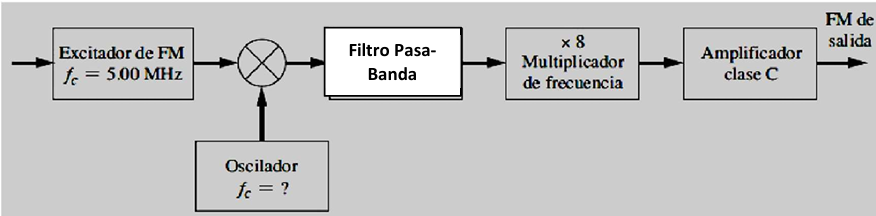
\includegraphics[width=0.8\textwidth]{imagenes/Parte_2/Actividad_11/fig4.png}
    \caption{Diagrama de bloques transmisor FM}
    \label{fig:4}
\end{figure}


\subsection*{a) Calcular el ancho de banda y la frecuencia central requerida para el filtro pasabanda.} 

El bloque multiplicador de frecuencia multiplica la frecuencia por un factor de 8.  
Por tanto, la frecuencia central del filtro pasabanda se calcula como:

    \[
        f_{central} = \frac{f_{sal}}{8} = \frac{97.9~[\text{MHz}]}{8} = 12.225~[\text{MHz}]
    \]

    \[
        \boxed{f_{central} = 12.225~[\text{MHz}]}
    \]

Como la desviación de frecuencia de salida es \(\Delta f_{sal} = 75~\text{kHz}\), entonces a la entrada del multiplicador:

    \[
        \Delta f_{exc} = \frac{\Delta f_{sal}}{8} = \frac{75~[\text{kHz}]}{8} = 9.375~[\text{kHz}]
    \]

    \[
        \boxed{f_{exc} = 9.375~[\text{MHz}]}
    \]

El ancho de banda se determina mediante la fórmula aproximada de Carson:
    \[
        B_T = 2(\Delta f + f_m) = 2(9.375~\text{kHz} + 15~\text{kHz}) = 48.75~[\text{kHz}]
    \]
    
    \[
        \boxed{B_T = 48.75~[\text{kHz}]}
    \]

\subsection*{b) Calcular la frecuencia $f_0$ del oscilador.}   

Al realizar el producto en el mezclador, se obtiene que:
    \[
        f_{exc} \pm f_{OL} = f_{central}
    \]

Reemplazando los valores:
    \[
        5~[\text{MHz}] \pm f_{OL} = 12.225~[\text{MHz}]
    \]

Para obtener la señal deseada a la salida del mezclador (en la frecuencia del filtro),se debe sumar la frecuencia del excitador con la del oscilador. Por lo tanto:
    
    \[
        f_{OL} = 12.225~[\text{MHz}] - 5~[\text{MHz}] = 7.225~[\text{MHz}]
    \]
    
    \[
        \boxed{f_{OL} = 7.225~[\text{MHz}]}
    \]

\subsection*{c) Determinar la capacidad de desviación pico requerida por el excitador de FM (que representa la salida ya modulada, desde un modulador de FM previo).}  

    \[
        \Delta f_{exc} = \frac{\Delta f_{sal}}{8} = \frac{75~[\text{kHz}]}{8} = 9.375~[\text{kHz}]
    \]
    \[
        \boxed{\Delta f_{exc} = 9.375~[kHz]}
    \]

Explicación:  Ni el mezclador ni el filtro alteran la desviación, solo el multiplicador de frecuencia modifica la escala.

\subsection*{d) Determinar el índice de modulación de la señal FM que se obtiene a la salida.}

    \[
        \beta = \frac{\Delta f_{sal}}{f_m} = \frac{75~[\text{kHz}]}{15~[\text{kHz}]} = 5
    \]
    \[
        \boxed{\beta = 5}
    \]


\subsection*{e) Indicar cómo es la separación de frecuencia de las frecuencias laterales adyacentes de esta señal FM de salida.}  

Las frecuencias laterales se encuentran sumando y restando múltiplos de la frecuencia modulante \( f_m \) a la portadora \( f_c \):

    \[
        f = f_c \pm n f_m, \quad n = 1, 2, 3, \dots
    \]

Para las dos primeras frecuencias laterales adyacentes:
    \[
        f_{1} = 97.9~[\text{MHz}] + 15~[\text{kHz}]
    \]
    \[
        f_{2} = 97.9~[\text{MHz}] - 15~[\text{kHz}]
    \]
    \[
        f_{1} = 97.885~[\text{MHz}]
    \]
    \[
        f_{2} = 97.915~[\text{MHz}]
    \]

Por lo tanto, la separación entre dos frecuencias laterales consecutivas (por ejemplo, entre la portadora y la primera lateral) siempre es igual a 
$f_m = 15~[kHz]$